% Options for packages loaded elsewhere
\PassOptionsToPackage{unicode}{hyperref}
\PassOptionsToPackage{hyphens}{url}
%
\documentclass[
  12pt,
]{article}
\usepackage{amsmath,amssymb}
\usepackage{iftex}
\ifPDFTeX
  \usepackage[T1]{fontenc}
  \usepackage[utf8]{inputenc}
  \usepackage{textcomp} % provide euro and other symbols
\else % if luatex or xetex
  \usepackage{unicode-math} % this also loads fontspec
  \defaultfontfeatures{Scale=MatchLowercase}
  \defaultfontfeatures[\rmfamily]{Ligatures=TeX,Scale=1}
\fi
\usepackage{lmodern}
\ifPDFTeX\else
  % xetex/luatex font selection
\fi
% Use upquote if available, for straight quotes in verbatim environments
\IfFileExists{upquote.sty}{\usepackage{upquote}}{}
\IfFileExists{microtype.sty}{% use microtype if available
  \usepackage[]{microtype}
  \UseMicrotypeSet[protrusion]{basicmath} % disable protrusion for tt fonts
}{}
\makeatletter
\@ifundefined{KOMAClassName}{% if non-KOMA class
  \IfFileExists{parskip.sty}{%
    \usepackage{parskip}
  }{% else
    \setlength{\parindent}{0pt}
    \setlength{\parskip}{6pt plus 2pt minus 1pt}}
}{% if KOMA class
  \KOMAoptions{parskip=half}}
\makeatother
\usepackage{xcolor}
\usepackage[margin=1in]{geometry}
\usepackage{graphicx}
\makeatletter
\def\maxwidth{\ifdim\Gin@nat@width>\linewidth\linewidth\else\Gin@nat@width\fi}
\def\maxheight{\ifdim\Gin@nat@height>\textheight\textheight\else\Gin@nat@height\fi}
\makeatother
% Scale images if necessary, so that they will not overflow the page
% margins by default, and it is still possible to overwrite the defaults
% using explicit options in \includegraphics[width, height, ...]{}
\setkeys{Gin}{width=\maxwidth,height=\maxheight,keepaspectratio}
% Set default figure placement to htbp
\makeatletter
\def\fps@figure{htbp}
\makeatother
\setlength{\emergencystretch}{3em} % prevent overfull lines
\providecommand{\tightlist}{%
  \setlength{\itemsep}{0pt}\setlength{\parskip}{0pt}}
\setcounter{secnumdepth}{-\maxdimen} % remove section numbering
\ifLuaTeX
  \usepackage{selnolig}  % disable illegal ligatures
\fi
\IfFileExists{bookmark.sty}{\usepackage{bookmark}}{\usepackage{hyperref}}
\IfFileExists{xurl.sty}{\usepackage{xurl}}{} % add URL line breaks if available
\urlstyle{same}
\hypersetup{
  pdftitle={LING 2200 Final Test},
  pdfauthor={Fall 2022},
  hidelinks,
  pdfcreator={LaTeX via pandoc}}

\title{LING 2200 Final Test}
\author{Fall 2022}
\date{/44pts}

\begin{document}
\maketitle

\hypertarget{name}{%
\section{Name:}\label{name}}

\hypertarget{student-number}{%
\section{Student number:}\label{student-number}}

You have the entire class period to complete this test. Please make all
answers on this exam booklet. For multiple choice and true/false
questions, circle the correct answer. You may use a calculator.

\textbf{Please show your work when necessary,} as partial credit will be
given based on it.

\begin{center}
Good luck!
\end{center}
\newpage

\hypertarget{a-15-newton-force-on-an-object-results-in-an-acceleration-of-5-ms2.-what-is-the-mass-of-the-object-please-provide-correct-units-2pts}{%
\subsubsection{\texorpdfstring{1. A 15 N(ewton) force on an object
results in an acceleration of 5 \(m/s^2\). What is the mass of the
object? Please provide correct units
{[}2pts{]}}{1. A 15 N(ewton) force on an object results in an acceleration of 5 m/s\^{}2. What is the mass of the object? Please provide correct units {[}2pts{]}}}\label{a-15-newton-force-on-an-object-results-in-an-acceleration-of-5-ms2.-what-is-the-mass-of-the-object-please-provide-correct-units-2pts}}

\[\\[2in]\]

\hypertarget{suppose-at-elevations-below-sea-level-p_atm-is-higher-than-at-sea-level.-if-youre-at-the-beach-and-you-dig-a-hole-1-mile-deep-then-jump-in-would-you-expect-the-vot-of-p-to-be-shorter-or-longer-than-if-you-were-at-sea-level-and-why-2pts}{%
\subsubsection{\texorpdfstring{2. Suppose at elevations below sea level
\(P_{atm}\) is higher than at sea level. If you're at the beach and you
dig a hole 1 mile deep then jump in, would you expect the VOT of /p/ to
be shorter or longer than if you were at sea level? and Why?
{[}2pts{]}}{2. Suppose at elevations below sea level P\_\{atm\} is higher than at sea level. If you're at the beach and you dig a hole 1 mile deep then jump in, would you expect the VOT of /p/ to be shorter or longer than if you were at sea level? and Why? {[}2pts{]}}}\label{suppose-at-elevations-below-sea-level-p_atm-is-higher-than-at-sea-level.-if-youre-at-the-beach-and-you-dig-a-hole-1-mile-deep-then-jump-in-would-you-expect-the-vot-of-p-to-be-shorter-or-longer-than-if-you-were-at-sea-level-and-why-2pts}}

\begin{enumerate}
\def\labelenumi{\alph{enumi}.}
\tightlist
\item
  Shorter because high pressure air released from the stop does not
  equalize the high \(P_{atm}\) quickly
\item
  Shorter because high pressure air released from the stop equalizes the
  high \(P_{atm}\) quickly
\item
  Longer because high pressure air released from the stop does not
  equalize the high \(P_{atm}\) quickly
\item
  Longer because high pressure air released from the stop equalizes the
  high \(P_{atm}\) quickly
\end{enumerate}

\hypertarget{a-balloon-is-filled-with-a-gas-that-has-a-volume-of-5-ml-at-3-atm-at-sea-level-will-have-what-volume-at-the-top-of-mt.-everest-where-the-pressure-drops-by-0.3-atm-give-your-answer-to-two-decimal-places-and-use-the-correct-units.-2pts}{%
\subsubsection{3. A balloon is filled with a gas that has a volume of 5
ml at 3 atm at sea level will have what volume at the top of Mt.
Everest, where the pressure drops by 0.3 atm? Give your answer to two
decimal places and use the correct units.
{[}2pts{]}}\label{a-balloon-is-filled-with-a-gas-that-has-a-volume-of-5-ml-at-3-atm-at-sea-level-will-have-what-volume-at-the-top-of-mt.-everest-where-the-pressure-drops-by-0.3-atm-give-your-answer-to-two-decimal-places-and-use-the-correct-units.-2pts}}

\[\\[2.5in]\]

\hypertarget{for-which-type-of-sound-wave-would-the-computation-of-rms-be-most-meaningful-as-a-measure-of-amplitude-1pt}{%
\subsubsection{4. For which type of sound wave would the computation of
RMS be most meaningful as a measure of amplitude?
{[}1pt{]}}\label{for-which-type-of-sound-wave-would-the-computation-of-rms-be-most-meaningful-as-a-measure-of-amplitude-1pt}}

\begin{enumerate}
\def\labelenumi{\alph{enumi}.}
\tightlist
\item
  Aperiodic waves
\item
  Sine waves
\item
  Complex periodic waves
\item
  Noise
\end{enumerate}

\hypertarget{below-are-two-sine-wave-equations-in-praat}{%
\subsubsection{5. Below are two sine wave equations in
Praat:}\label{below-are-two-sine-wave-equations-in-praat}}

0.25 * sin(2 * pi * 377 * x)

0.75 * sin(2 * pi * 377 * x)

What is the RMS amplitude of the resulting wave when the two waves are
added? Round your answer to the twp digits. {[}2pts{]}

\[\\[1in]\]

\hypertarget{the-tines-of-a-tuning-fork-move-back-and-forth-400-times-a-second.-what-is-the-period-in-milliseconds-of-the-resulting-sine-wave-use-correct-units.1pt}{%
\subsubsection{6. The tines of a tuning fork move back and forth 400
times a second. What is the period (in milliseconds) of the resulting
sine wave? Use correct
units.{[}1pt{]}}\label{the-tines-of-a-tuning-fork-move-back-and-forth-400-times-a-second.-what-is-the-period-in-milliseconds-of-the-resulting-sine-wave-use-correct-units.1pt}}

\[\\[1in]\]

\hypertarget{would-a-100-hz-tone-played-outside-at-the-equator-in-the-summer-would-have-a-wavelength-longer-than-a-100-hz-tone-played-outside-in-toronto-in-the-winter-yes-or-no-and-why-2pts}{%
\subsubsection{7. Would a 100 Hz tone played outside at the equator in
the summer would have a wavelength longer than a 100 Hz tone played
outside in Toronto in the winter? Yes or No, and why?
{[}2pts{]}}\label{would-a-100-hz-tone-played-outside-at-the-equator-in-the-summer-would-have-a-wavelength-longer-than-a-100-hz-tone-played-outside-in-toronto-in-the-winter-yes-or-no-and-why-2pts}}

\[\\[2in]\]

\hypertarget{is-the-following-statement-true-or-false-the-glottal-spectrum-of-a-high-pitched-female-would-have-energy-missing-in-more-frequencies-than-a-low-pitched-male-glottal-spectrum.-2pts}{%
\subsubsection{8. Is the following statement true or false: The glottal
spectrum of a high-pitched female would have energy missing in more
frequencies than a low-pitched male glottal spectrum.
{[}2pts{]}}\label{is-the-following-statement-true-or-false-the-glottal-spectrum-of-a-high-pitched-female-would-have-energy-missing-in-more-frequencies-than-a-low-pitched-male-glottal-spectrum.-2pts}}

TRUE / FALSE

Explain your answer:

\[\\[1in]\]

\hypertarget{below-is-a-hypotheical-glottal-spectrum.-what-is-the-frequency-and-amplitude-of-the-harmonic-marked-triangle-4pts}{%
\subsubsection{\texorpdfstring{9. Below is a hypotheical glottal
spectrum. What is the \textbf{frequency} and \textbf{amplitude} of the
harmonic marked \(\triangle\) ?
{[}4pts{]}}{9. Below is a hypotheical glottal spectrum. What is the frequency and amplitude of the harmonic marked \textbackslash triangle ? {[}4pts{]}}}\label{below-is-a-hypotheical-glottal-spectrum.-what-is-the-frequency-and-amplitude-of-the-harmonic-marked-triangle-4pts}}

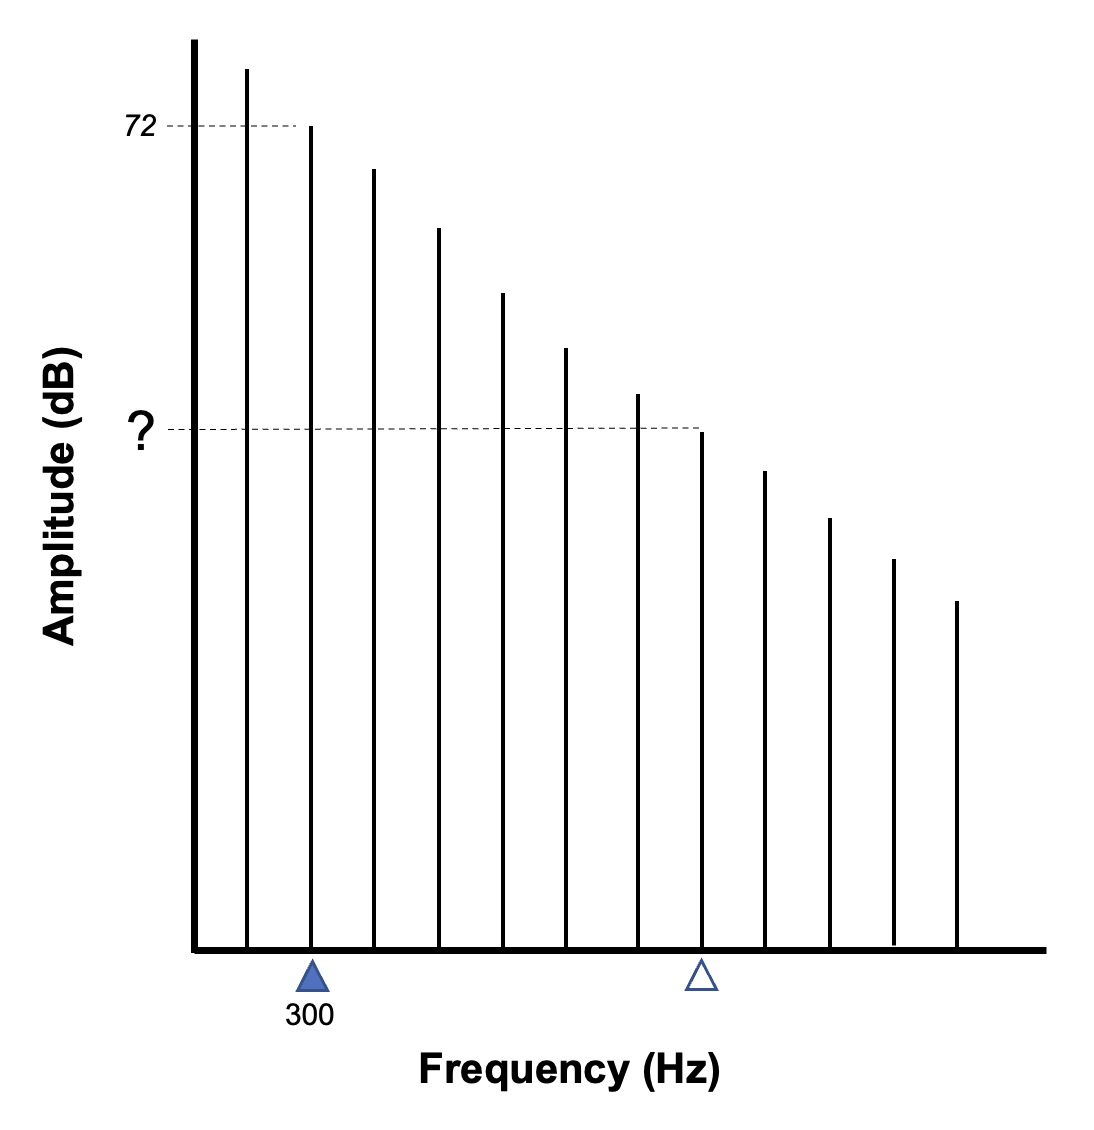
\includegraphics[width=0.5\textwidth,height=0.5\textheight]{images/glottal_spec_fin.png}

\hypertarget{frequency}{%
\subsection{Frequency=}\label{frequency}}

\hypertarget{amplitude}{%
\subsection{Amplitude=}\label{amplitude}}

\pagebreak

\hypertarget{the-basilar-membrane-is-characterized-by-its-tonotopic-organization-which-decomposes-the-incoming-complex-periodic-wave-into-its-component-frequencies.-what-is-tonotopic-organization-comparable-to-1pt}{%
\subsubsection{\texorpdfstring{10. The basilar membrane is characterized
by its \emph{tonotopic} organization, which decomposes the incoming
complex periodic wave into its component frequencies. What is tonotopic
organization comparable to?
{[}1pt{]}}{10. The basilar membrane is characterized by its tonotopic organization, which decomposes the incoming complex periodic wave into its component frequencies. What is tonotopic organization comparable to? {[}1pt{]}}}\label{the-basilar-membrane-is-characterized-by-its-tonotopic-organization-which-decomposes-the-incoming-complex-periodic-wave-into-its-component-frequencies.-what-is-tonotopic-organization-comparable-to-1pt}}

\begin{enumerate}
\def\labelenumi{\alph{enumi}.}
\tightlist
\item
  Categorical perception
\item
  Fourier analysis
\item
  Perceptual magnet effect
\item
  Quarter-wave resonator
\end{enumerate}

\hypertarget{why-does-the-k-in-coo-sound-different-from-the-k-in-key-and-what-phenomenon-is-it-the-result-of-2pts}{%
\subsubsection{11. Why does the ``k'' in ``coo'' sound different from
the ``k'' in ``key, and what phenomenon is it the result of?
{[}2pts{]}}\label{why-does-the-k-in-coo-sound-different-from-the-k-in-key-and-what-phenomenon-is-it-the-result-of-2pts}}

\begin{enumerate}
\def\labelenumi{\alph{enumi}.}
\tightlist
\item
  Lips are rounded in ``coo'' and as a result the oral cavity is
  lengthened, raising F1; segmentation
\item
  Lips are rounded in ``coo'' and as a result the pharyngeal cavity is
  widened, raising F2; coarticulation
\item
  Lips are rounded in ``coo'' and as a result the oral cavity is
  lengthened, lowering F2; coarticulation
\item
  The tongue is further back in ``coo'' and as a result the oral cavity
  is lengthened, lowering F2; coarticulation
\end{enumerate}

\hypertarget{suppose-you-have-a-hole-at-the-roof-of-your-mouth-cleft-palate.-1-why-cant-you-make-a-stop-consonant-2pts}{%
\subsubsection{12. Suppose you have a hole at the roof of your mouth
(cleft palate). 1) Why can't you make a stop consonant?
{[}2pts{]}}\label{suppose-you-have-a-hole-at-the-roof-of-your-mouth-cleft-palate.-1-why-cant-you-make-a-stop-consonant-2pts}}

\[\\[2in]\]

BONUS:How do you propose you can make a stop consonant sound and why
would this work? {[}1pt{]} Write your answer below.

\[\\[1.5in]\]

\hypertarget{what-is-the-db-value-for-a-sound-with-an-absolute-intensity-of-0.0053-wm2-round-your-answer-to-two-decimal-places.3pts}{%
\subsubsection{\texorpdfstring{13. What is the dB value for a sound with
an absolute intensity of 0.0053 \(W/m^2\)? Round your answer to two
decimal
places.{[}3pts{]}}{13. What is the dB value for a sound with an absolute intensity of 0.0053 W/m\^{}2? Round your answer to two decimal places.{[}3pts{]}}}\label{what-is-the-db-value-for-a-sound-with-an-absolute-intensity-of-0.0053-wm2-round-your-answer-to-two-decimal-places.3pts}}

\[\\[3.5in]\]

\hypertarget{suppose-you-have-a-tube-thats-closed-at-one-end.-the-frequency-of-the-3rd-resonance-is-0.054khz.-assuming-that-the-speed-of-sound-is-330ms-what-is-the-length-of-the-tube-in-cm-use-correct-units.3pts}{%
\subsubsection{14. Suppose you have a tube that's closed at one end. The
frequency of the 3rd resonance is 0.054kHz. Assuming that the speed of
sound is 330m/s, what is the length of the tube in cm? Use correct
units.{[}3pts{]}}\label{suppose-you-have-a-tube-thats-closed-at-one-end.-the-frequency-of-the-3rd-resonance-is-0.054khz.-assuming-that-the-speed-of-sound-is-330ms-what-is-the-length-of-the-tube-in-cm-use-correct-units.3pts}}

\[\\[3.5in]\]

\hypertarget{below-are-the-f1-and-f2-values-for-the-same-vowel-spoken-by-a-man-woman-and-child.-what-is-the-f1-value-that-we-should-expect-the-child-to-have-given-the-measurements-of-the-two-adults-use-correct-units.-show-your-work.-2pts}{%
\subsubsection{\texorpdfstring{15.Below are the F1 and F2 values for the
\textbf{same vowel} spoken by a Man, Woman, and Child. What is the F1
value that we should expect the child to have given the measurements of
the two adults? Use correct units. Show your work.
{[}2pts{]}}{15.Below are the F1 and F2 values for the same vowel spoken by a Man, Woman, and Child. What is the F1 value that we should expect the child to have given the measurements of the two adults? Use correct units. Show your work. {[}2pts{]}}}\label{below-are-the-f1-and-f2-values-for-the-same-vowel-spoken-by-a-man-woman-and-child.-what-is-the-f1-value-that-we-should-expect-the-child-to-have-given-the-measurements-of-the-two-adults-use-correct-units.-show-your-work.-2pts}}

Man: F1 = 570Hz; F2 = 1995Hz\\
Woman: F1 = 689Hz; F2 = 2411Hz\\
Child: F1 = ?; F2 = 2450Hz

\hypertarget{f1-child}{%
\subsection{F1 (child) =}\label{f1-child}}

\[\\[1.5in]\]

\hypertarget{which-is-the-more-broadly-tuned-filter-1pt}{%
\subsubsection{16. Which is the more broadly tuned filter?
{[}1pt{]}}\label{which-is-the-more-broadly-tuned-filter-1pt}}

\begin{enumerate}
\def\labelenumi{\alph{enumi}.}
\tightlist
\item
  Straight open-closed tube
\item
  Vocal tract
\end{enumerate}

\hypertarget{why-is-the-high-front-vowel-usually-produced-with-lip-spreading-2pts}{%
\subsubsection{17. Why is the high front vowel usually produced with
lip-spreading?
{[}2pts{]}}\label{why-is-the-high-front-vowel-usually-produced-with-lip-spreading-2pts}}

\[\\[1in]\]

\hypertarget{which-of-the-following-is-not-an-indication-of-phonological-voicing-in-initial-stop-consonants-before-a-vowel-1pt}{%
\subsubsection{\texorpdfstring{18. Which of the following is
\textbf{not} an indication of phonological voicing in initial stop
consonants before a vowel?
{[}1pt{]}}{18. Which of the following is not an indication of phonological voicing in initial stop consonants before a vowel? {[}1pt{]}}}\label{which-of-the-following-is-not-an-indication-of-phonological-voicing-in-initial-stop-consonants-before-a-vowel-1pt}}

\begin{enumerate}
\def\labelenumi{\alph{enumi}.}
\tightlist
\item
  Onset timing and frequency of the second formant
\item
  VOT
\item
  Onset timing and frequency of the first formant
\item
  Fundamental frequency of the vowel
\end{enumerate}

\pagebreak

\hypertarget{below-are-two-spectra-of-sibilant-fricatives.-one-is-s-and-the-other-is-sh.-which-is-which-and-how-can-you-tell-2pts}{%
\subsubsection{19. Below are two spectra of sibilant fricatives. One is
{[}s{]} and the other is {[}sh{]}. Which is which, and how can you tell?
{[}2pts{]}}\label{below-are-two-spectra-of-sibilant-fricatives.-one-is-s-and-the-other-is-sh.-which-is-which-and-how-can-you-tell-2pts}}

\hypertarget{left}{%
\subsection{Left =}\label{left}}

\hypertarget{right}{%
\subsection{Right =}\label{right}}

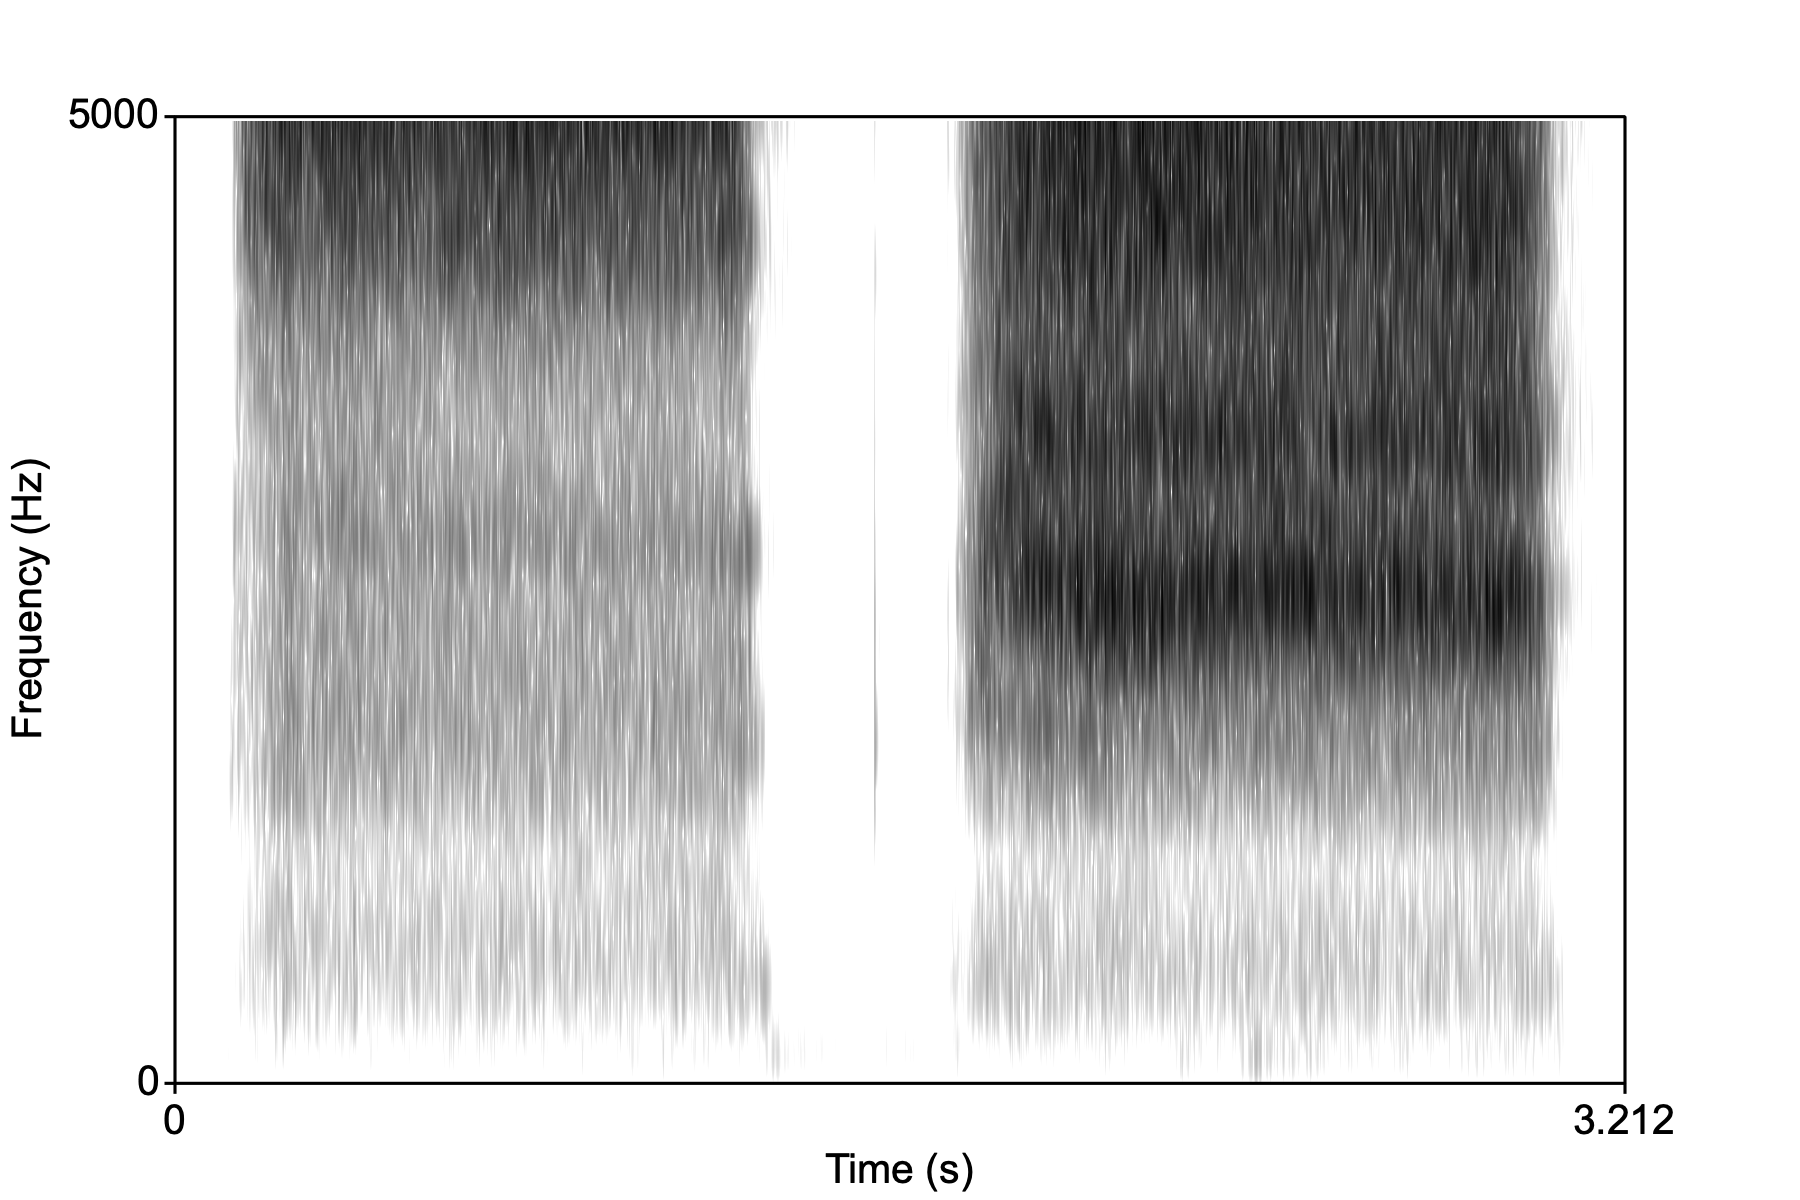
\includegraphics[width=0.5\textwidth,height=0.5\textheight]{images/sibilants_fin.png}

Explain: \[\\[1in]\]

\hypertarget{is-the-following-statement-true-or-false-the-intraoral-pressure-of-short-or-zero-vot-consonants-is-lower-than-positive-vot-consonants.-1pt}{%
\subsubsection{20. Is the following statement true or false: The
intraoral pressure of short (or zero) VOT consonants is lower than
positive VOT consonants.
{[}1pt{]}}\label{is-the-following-statement-true-or-false-the-intraoral-pressure-of-short-or-zero-vot-consonants-is-lower-than-positive-vot-consonants.-1pt}}

TRUE / FALSE

BONUS: Explain your answer.{[}2pts{]}

\[\\[2in]\]

\hypertarget{match-the-two-window-lengths-to-the-spectrograms-below-label-the-spectrograms-as-a-or-b-1pt}{%
\subsubsection{21. Match the two window lengths to the spectrograms
below (label the spectrograms as ``a'' or ``b'')
{[}1pt{]}:}\label{match-the-two-window-lengths-to-the-spectrograms-below-label-the-spectrograms-as-a-or-b-1pt}}

\begin{enumerate}
\def\labelenumi{\alph{enumi}.}
\tightlist
\item
  0.005s
\item
  0.05s
\end{enumerate}

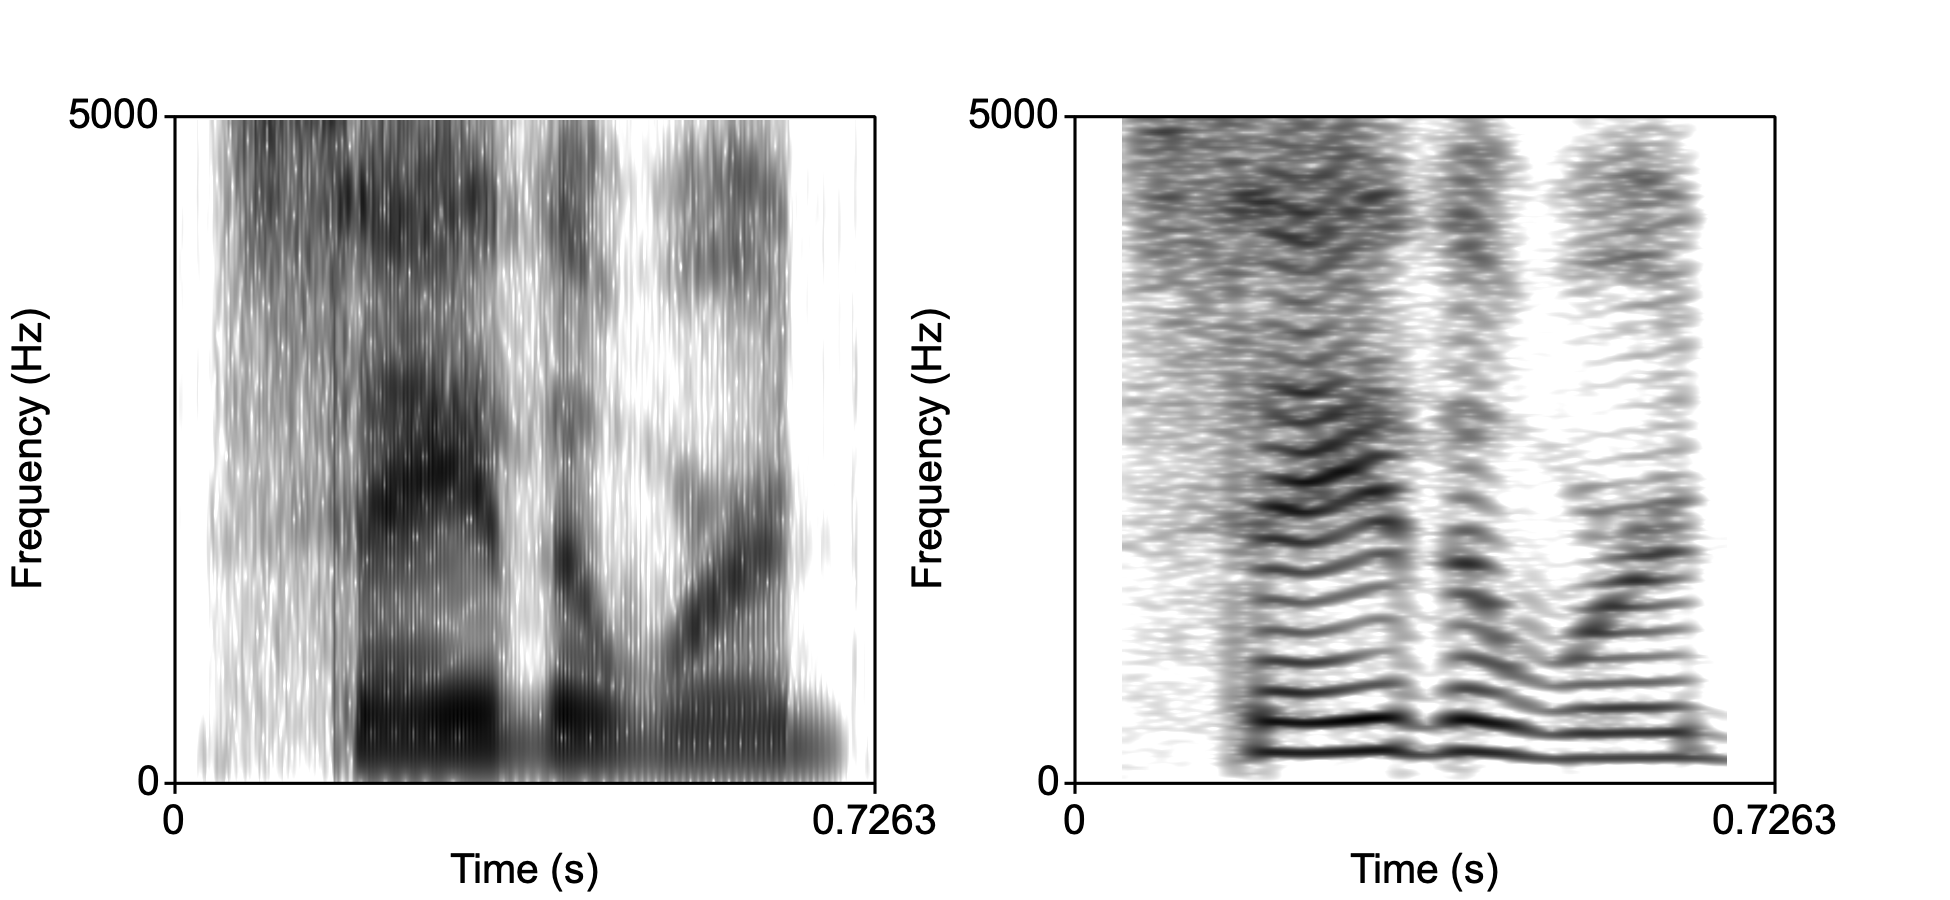
\includegraphics{images/wide_narrow_fin.png}

Explain your answer {[}2pts{]}:

\[\\[1.5in]\]

\hypertarget{the-fact-that-japanese-quail-can-perceive-speeech-sounds-categorically-was-a-problem-for-the-motor-theory.-why-3pts}{%
\subsubsection{22. The fact that Japanese Quail can perceive speeech
sounds categorically was a problem for the Motor Theory. Why?
{[}3pts{]}}\label{the-fact-that-japanese-quail-can-perceive-speeech-sounds-categorically-was-a-problem-for-the-motor-theory.-why-3pts}}

\[\\[2in]\]

\end{document}
